\documentclass[dvipsnames]{standalone}

\usepackage{tikz}
\usetikzlibrary{shapes, arrows, positioning,backgrounds,scopes, calc, fit}
\usepackage{xcolor}
\usepackage{pdfpages}


\pgfdeclarelayer{background}
\pgfsetlayers{background,main}
	
\pgfmathsetmacro{\myinnersep}{2}% inner sep in mm
	
\newcommand{\iconbox}[2]{\begin{minipage}{6cm}
\centering
    #1\par
    \includegraphics[height=2cm]{#2}
    \end{minipage}
}
	
\begin{document}
\begin{tikzpicture}
    [dline/.style={-triangle 45, line width=5, font=\Huge},
    dnode/.style={fill=white, font=\Huge},
    gicon/.style={dnode, draw, rounded corners=0.05cm, minimum height=3cm, minimum width=6cm, align=center, inner sep=\myinnersep},
    software/.style={dnode, fill=gray!20, font=\itshape\Huge, rounded corners=0.1cm, minimum width=9cm},
    slabel/.style={below right, font=\bfseries\Huge}] 
    \begin{scope}[scale=1]
    
        \node[] (spread-title) {\Huge{Spreadsheet Software}};
        \node[gicon, below=of spread-title.west, anchor=north east, xshift= -2cm, minimum height=2cm, inner sep=\myinnersep] (edit) {
\includegraphics[width=2cm]{images/icons/edit}};
        \node[gicon, below=of spread-title.east, anchor=north west, xshift=  2cm, minimum height=2cm, inner sep=\myinnersep] (view) {
\includegraphics[width=2cm]{images/icons/view}};
        
        \begin{pgfonlayer}{background}    % select the background layer
            \node[software, minimum width=1cm, fit={(spread-title) (edit) (view)}] (spread) {};
        \end{pgfonlayer}
        
        \node[gicon, below=4cm of spread-title] (convert) {\iconbox{Convert (F1)}{images/guigraphics/convertodml}};
        \node[gicon, below=of convert.south east, xshift=1cm] (compare){\iconbox{Compare (F3)}{images/guigraphics/comparetable}};
        \node[gicon, right=of compare] (merge) {\iconbox{Merge (F4)}{images/guigraphics/mergeodml}};
        \node[gicon, right=of merge] (filter) {\iconbox{Filter (F5)}{images/guigraphics/filterodml}};
        \node[gicon] (empty) at ($(edit |- compare)$) {\iconbox{Template (F2)}{images/guigraphics/createtemplate}};
        \node[left=of empty, anchor=south east] (odt-logo) {
\includegraphics[width=4cm]{images/logos/odMLtables}};
        
        \begin{pgfonlayer}{background}
            \node[software, fit={(odt-logo) (empty) (compare) (merge) (filter) (convert)}] (odt) {};
            \node[slabel] at (odt.north west) {odMLtables};
        \end{pgfonlayer}
        
        \node[software, below=2cm of filter.south east, xshift=1cm] (odml) {
\includegraphics[height=2cm]{images/logos/odmLogo}};
        \node[slabel] at (odml.north west) {odML};
        \node[software, below=of odml.south, anchor=north west, xshift=1.5cm, minimum height=2cm] (neo) {\hspace{1.5cm}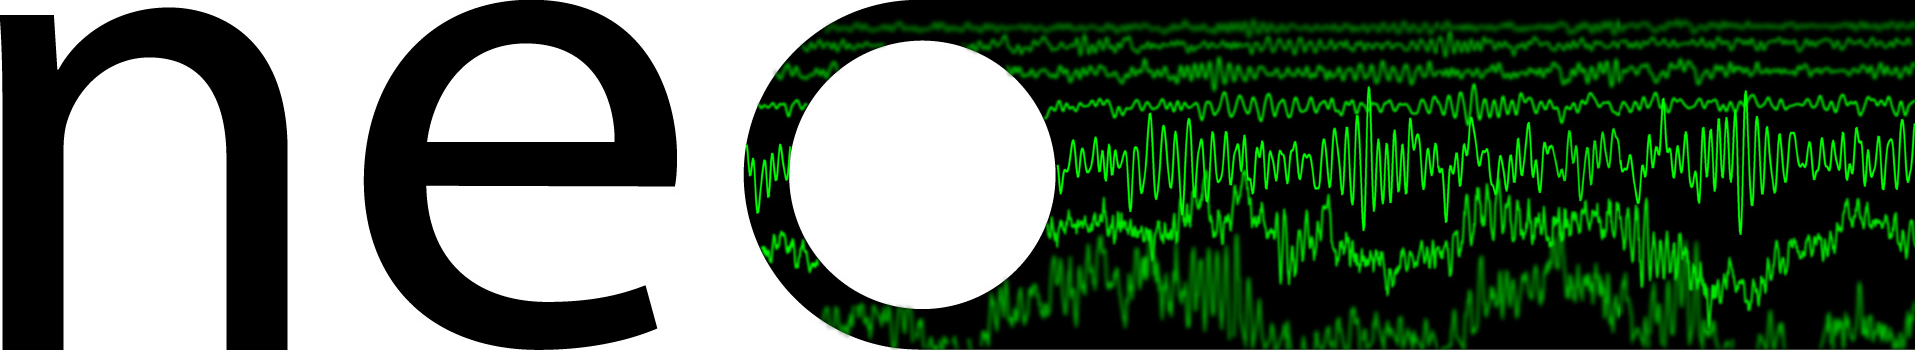
\includegraphics[height=1.2cm]{images/logos/neologo_alpha3}};
        \node[slabel] at (neo.north west) {Neo};
        \node[software, below=of neo.south, anchor=north west, xshift=1.5cm] (nix) {
\includegraphics[height=2cm]{images/logos/NixLogo}};
        \node[slabel] at (nix.north west) {NIX};
        \node[below=of nix.south east, anchor=north west] (db-text) {\Huge{Database}};
        \node[below=of db-text.south, anchor=center] (db-logo) {
\includegraphics[height=2cm]{images/icons/database}};
        \begin{pgfonlayer}{background}
            \node[software,fit={(db-text) (db-logo)}] (db) {};
        \end{pgfonlayer}
        
        \draw[dline] (empty.north) -- (edit.south);
        \draw[dline] (edit.east) --++ (1,0) |- (convert.west);
        \draw[dline, dashed] (convert.north) |- (view.west);
        \draw[dline] (convert.east) -| (odml.north);
        \draw[dline, dashed] (compare.north) --++ (0,4) -| (view.south);
        \draw[dline, -] (merge.north) |- (convert.east);
        \draw[dline, -] (filter.north) |- (convert.east);
        \draw[dline] (odml.west) -| (compare.south);
        \draw[dline] (odml.west) -| (merge.south);
        \draw[dline] (odml.west) -| (convert.south);
        \begin{pgfonlayer}{background}
            \draw[dline] (odml) -| (filter.south);
        \end{pgfonlayer}
        
        \draw[dline] (odml.south) |- (neo.west);
        \draw[dline] (odml.south) |- node[near start, left] {
\includegraphics[height=2cm]{images/icons/hand}} (nix.west);
        \draw[dline] (nix.south) |- (db.west);
        \draw[dline] (odml.east) -| (db.north);
        
        
        \coordinate (t0) at ($(odt.west |- db.south) + (0,-2)$);
        \coordinate (t1) at (t0 -| db.east);
        
        
        % add time axis
        \draw[dline] (t0) -- (t1) {};
%         \node[above=of t1, anchor=center] {\Huge{Time}};
        \node[above=of t0, anchor=center] {\Huge{Experiment}};
        
        \node[below=of t0, xshift=3cm, anchor=north west] (prep) {\Huge{Preparation}};
        \node[right=10cm of prep] (cond) {\Huge{Execution}};
        \node[right=10cm of cond] (rep) {\Huge{Report}};
        \node[below=of rep] (doc) {\Huge{Documentation}};
        \node[right=10cm of rep] (ana) {\Huge{Analysis}};
        \node[right=10cm of ana] (share) {\Huge{Sharing}};
        \node[below=of share] (pub) {\Huge{Publication}};
        \node[below=of pub] () {\Huge{Indexing}};
        
    \end{scope}
\end{tikzpicture}
\end{document}
